\documentclass[aspectratio=169,compress,10pt]{beamer}
\usepackage[utf8]{inputenc}
\usepackage[T1]{fontenc}
\usepackage{lipsum, lmodern}
\usepackage{textcomp}
\usepackage{algorithm}
\usepackage{algorithmic}
\usetheme{Szeged} % or Median, or Metro, or PraterStreet, or Milano

\usecolortheme{spruce}

\author{Rafael Pérez-Torres}
\title{Re-sampling and cross-validation}
\institute{Cinvestav Tamaulipas}
\date{\today}

\begin{document}
\frame{\maketitle}
\begin{frame}{Table of contents}
	\tableofcontents
\end{frame}

\section{Introduction}
\begin{frame}{Introduction}

{\Large{} Why cross validation and resampling?} 

Cross-validation and resampling methods are validation techniques helpful for:
\begin{itemize}
	\item Selecting model.
	\begin{itemize}
		\item Almost all pattern recognition techniques needs one or more parameters.
		\item How to select the \emph{optimal} parameters?
	\end{itemize}
	\item Classifiers performance evaluation.
	\begin{itemize}
		\item Once the model is selected, how to estimate its performance?
		\item The goal is the real error rate, but this is only achievable by performing classification over the whole population.
	\end{itemize}
\end{itemize}
\end{frame}

\begin{frame}{Introduction}

{\Large{} Why cross-validation and resampling?} 

\begin{itemize}
	\item Usually the available dataset size is not as large as we would want.
	\item One approach would be selecting the entire dataset for the classifier training and evaluation, but:
	\begin{itemize}
		\item This would overfit training data.
		\item The error rate estimate might be really optimistic.
	\end{itemize}
\end{itemize}

{\Large{} Resampling and cross-validation techniques to the rescue!} 
\end{frame}

\section{Cross-validation techniques}
\subsection{Description}
\begin{frame}{Cross-validation techniques}
% {\Large{} Hold out cross validation} 
\begin{itemize}
	\item Basically, they divide available dataset on two global subsets, one for training, the other for testing the classifier.
	\item Subsets are mutually exclusive, the instance $x_i$ can be only in one of these subsets.
\end{itemize}
\end{frame}

\subsection{Holdout cross-validation}
\begin{frame}{Holdout cross-validation}
\begin{itemize}
	\item It divides the dataset into the training and testing subsets.
	\item Usually, $2/3$ for training, $1/3$ for testing.
	\item A typical usage of holdout is determining a stopping point for the back propagation error in ANN.
\end{itemize}
\centering
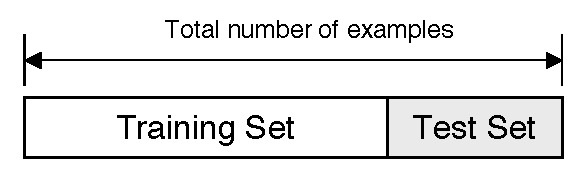
\includegraphics[width=0.5\textwidth]{../report/resources/images/holdout}
\end{frame}

\begin{frame}{Holdout cross-validation}

{\Large{} Drawbacks} 

\begin{itemize}
	\item For small datasets it is not possible to set aside a portion of the dataset for testing.
	\item It is a single  train-and-test experiment, the estimation of error might be unrealistic.
	\item There are several alternatives to overcome these issues.
\end{itemize}
\end{frame}

\subsection{K-fold cross-validation}
\begin{frame}{K-fold cross-validation}
\begin{itemize}
	\item Split the dataset in $k$ folds.
	\item For each $k$ experiments, use $k-1$ folds for training and the remaining one for testing.
	\item All instances in the dataset are eventually used for both training and testing.
	\item The estimation of the true error is the average error rate:
$$
	E = \frac{1}{k} \sum_{i=1}^k E_{i}
$$
\end{itemize}
\centering{}
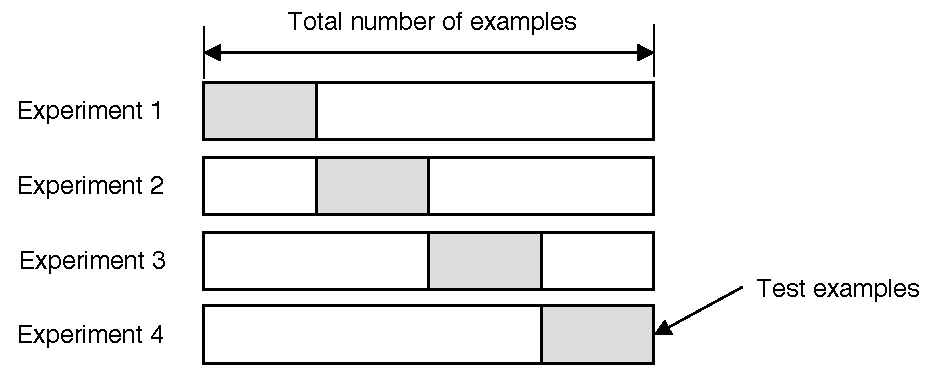
\includegraphics[width=0.5\textwidth]{../report/resources/images/k-fold}
\end{frame}


\begin{frame}{K-fold cross-validation}

{\Large{} How many folds?} 

For a large number of folds:
\begin{itemize}
	\item \checkmark The bias of the true error rate estimator will be small .
	\item \texttimes The variance of the true error rate estimator will be large.
	\item \texttimes The computational time will be very large as well (many experiments).
\end{itemize}

For a small number of folds:
\begin{itemize}
	\item \checkmark The number of experiment and computation time are reduced.
	\item \checkmark The variance of estmator will be small.
	\item \texttimes The bias of estimator will be large.
\end{itemize}

For very sparse datasets, leave-one-out cross validation is preferred in order to train on as many examples as possible.
A common choice for K is 10.
\end{frame}


\subsection{Leave-one-out cross-validation}

\begin{frame}{Leave-one-out cross-validation}
\begin{itemize}
	\item Special case of the K-cross validation, where $k =$ number of instances.
	\item For a dataset with $N$ instances, perform $N$ experiments.
	\item In each experiment use $N-1$ instances for training and the remaining one for testing.
	\item The estimation of the true error is the average error rate:
$$
	E = \frac{1}{n} \sum_{i=1}^n E_{i}
$$
\end{itemize}
\centering{}
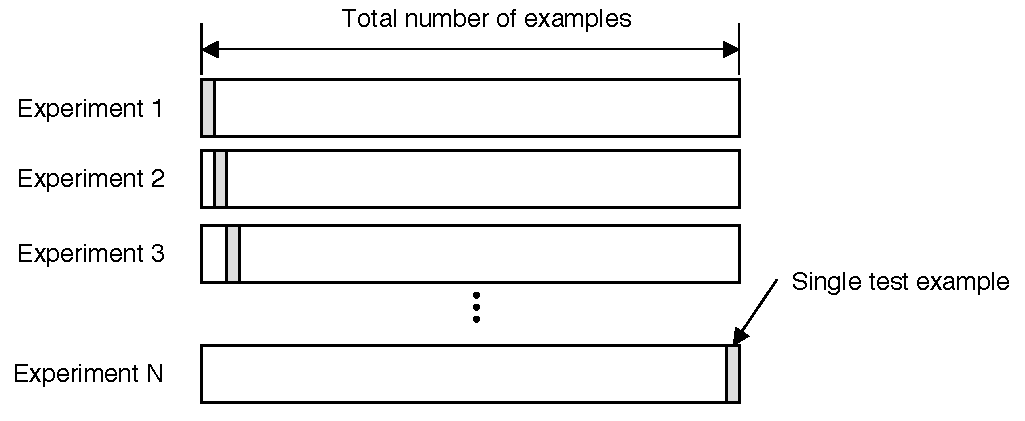
\includegraphics[width=0.5\textwidth]{../report/resources/images/leave-one-out}
\end{frame}


\section{Re-sampling techniques}
\subsection{Description}
\begin{frame}{Re-sampling techniques}
% {\Large{} Hold out cross validation} 
\begin{itemize}
	\item Split dataset in subsets employing sampling with replacement.
	\item In this way, an instance can appear in more than one subset and more than once.
\end{itemize}
\end{frame}

\subsection{Bootstrap family}
\begin{frame}{Bootstrap family}
\begin{itemize}
	\item The bootstrap techniques family employs a dataset with $n$, samples it with replacement, creating several \emph{syntethic} datsets of size $n$, too.
	\item For obtaining the real error rate, classification is launched with the synthetic datasets created, and further processing the error results.
	\item In practice, this re-sampling strategy works because if samples are randomly selected, they will keep the same features of the population they came from.
\end{itemize}
\end{frame}

\begin{frame}{Bootstrap real error rate estimation}
\begin{itemize}
	\item If trainind dataset is $\mathbf{X} = (x_1,\ldots,x_N)$ then , it is possible to collect $\mathcal{B}$ bootstrap samples with replacement $\mathbf{Z_1}, \ldots, \mathbf{Z_B}$ where each $\mathbf{Z_i}$ contains $n$ instances.
	\item Then, it is possible to employ the set $\mathbf{Z}$ for estimating the real error rate in classifier prediction as:
$$
\text{Err}_{\text{boot}} = \frac{1}{B} \sum_{b=1}^{B} \frac{1}{N} \sum_{i=1}^{N} \mathcal{L}(y_i, f^b(x_i))
$$
where $f^b(x_i)$ is the predicted value for $x_i$ according to the model generated for the $i$ bootstrap dataset, and $\mathcal{L}$ is an error measurement function.
\end{itemize}
\end{frame}

\subsection{LOOB}
\begin{frame}{L-O-O Bootstrap real error rate estimation}
\begin{itemize}
	\item Previous estimator is not optimal since the samples employed for training the classifier might had contained $x_i$.
	\item The leave-one-out bootstrap estimator improves this, trying to imitate the cross-validation approach.
	\item The LOOB estimator is defined as:
	$$
	\text{Err}_{\text{boot(1)}} = \frac{1}{N} \sum_{i=1}^N \frac{1}{|C^{-1}|} \sum_{b \in C^{-i}} \mathcal{L}(y_i, f^b(x_i))
	$$
	where $C^{-i}$ is the index set of bootstrap sets that do not contain the instance $i$ and $|C^{-i}|$ is the amount of such sets. 
\end{itemize}
\end{frame}


\subsection{Bootstrap .632}
\begin{frame}{Bootstrap .632 real error rate estimation}
\begin{itemize}
	\item $\text{Err}_{\text{boot(1)}}$ fixes overfitting problem but still exposes a bias created by non-distinct observations of the sampling with replacement strategy.
	\item It has been calculated that the average of distinct instances in wach bootstrap set is approximately $0.632N$.
	\item Efron and Tibshirani proposed the bootstrap $0.632$ error rate estimator, defined as:
	\begin{equation}
		\text{Err}_{.632} = 0.368 \overline{\text{err}} + 0.632 \text{Err}_{\text{boot}(1)}
		\label{eq:bootstrap}
	\end{equation}
	where
	$$
	\overline{\text{err}} = \frac{1}{N} \sum_{i=1}^{N} \mathcal{L}(y_i,f^b(x_i))
	$$
	\item This formulation can be generalized as:
	\begin{equation}
		\text{Err}_{.632} = w \overline{\text{err}} + (1 - w) \text{Err}_{\text{boot}(1)}
	\end{equation}
	where $w=0.368$.
\end{itemize}
\end{frame}

\subsection{Bootstrap .632+}
\begin{frame}{Bootstrap .632+ real error rate estimation}
\begin{itemize}
	\item Under certain scenarios, bootstrap .632 still can describe a large overfitting, when the resubstitution error ($\text{Err}_{\text{boot}(1)}$) is $0$.
	\item The \emph{bootstrap .632+} real error rate estimator puts a larger weight $w$ over $\text{Err}_{\text{boot}(1)}$.
	\item The $w$ weight is calculated from the \emph{relative overlapping rate} $\hat{R}$ as
	$$
	\hat{R} = \frac{\overline{\text{err}} - \text{Err}_{\text{boot}(1)}}{\hat{\gamma} - \text{Err}_{\text{boot}(1)}}
	$$
	where
	$\hat{\gamma}$ is the \emph{no-information error rate}.
\end{itemize}
\end{frame}

\begin{frame}{Bootstrap .632+ real error rate estimation}
\begin{itemize}
	\item $\hat{\gamma}$ ( the \emph{no-information error rate}) can be estimated through the permutation of answers $y_i$ and the predictors (patterns) $t_j$.
	\item In a dicotomic classification problem, the no-information rate can be calculated as follows:
	\begin{itemize}
		\item Let $\hat{p}_1$ the proportion of answers $y_i = 1$  and $\hat{q}_1$ the proportion of observed predictions $r_x(t_j) = 1$, then:
		$$
			\hat{\gamma} = \hat{p}_1(1-\hat{q}_1) + (1-\hat{p}_1) \hat{q}_1
		$$
	\end{itemize}
\end{itemize}
\end{frame}

\begin{frame}{Bootstrap .632+ real error rate estimation}
\begin{itemize}
	\item Finally, the bootstrap .632+ real error rate estimation is defined as:
	\begin{equation}
		\text{Err}_{.632+} = w \overline{\text{err}} + (1 - w) \text{Err}_{\text{boot}(1)}, \text{ } w = \frac{.632}{1-.368\hat{R}}
	\end{equation}
	\item This estimator is highly realiable when $n>p$ (there are more instances than attributes - dimensions).
\end{itemize}
\end{frame}


\section{Three-way data splits}
\subsection{Description}
\begin{frame}{Three-way data splits}
If model selection and estimation of error need to be computed simultaneously, the data needs to be divided into three disjoint sets:
\begin{itemize}
	\item \textbf{Training set}: A set of examples used for learning and fitting the parameters of the classifier.
	\item \textbf{Validation set}: A set of examples used to tune the parameters of a classifier.
	\item \textbf{Testing set}: A set of instances used \textbf{only} to assess the performance of a fully trained classifier.
\end{itemize}

\end{frame}

\subsection{Basic methodology}
\begin{frame}{Three-way data splits}
\centering{}
%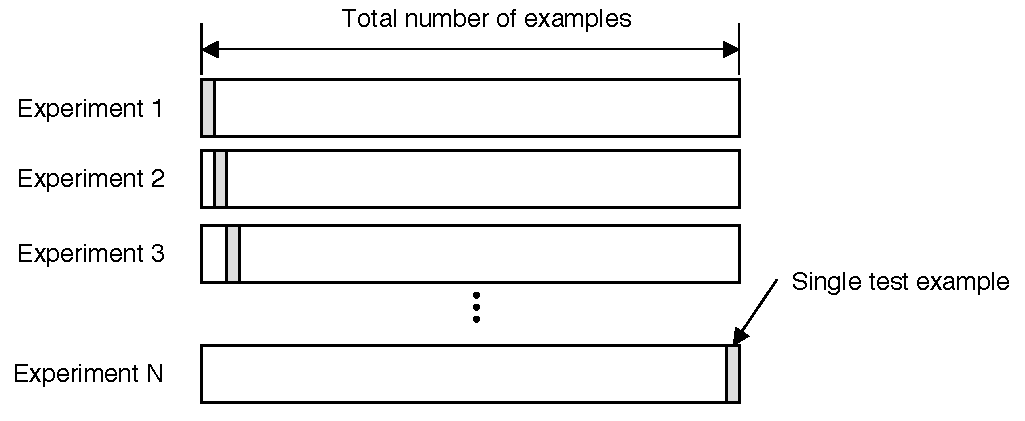
\includegraphics[width=0.5\textwidth]{../report/resources/images/leave-one-out}
\begin{algorithmic}[1] 
\STATE Divide the available data into training, validation and test set.
\STATE Select architecture and training parameters. \label{paso-2}
\STATE Train the model using the training set.
\STATE Evaluate the model using the validation set. \label{paso-4}
\STATE Repeat steps \ref{paso-2} through \ref{paso-4} using different architectures and training parameters.
\STATE Select the best model and train it using data from the training and validation set.
\STATE Assess this final model using the test set.
\end{algorithmic} 

If CV or bootstrap are used, steps 3 and 4 have to be repeated for each of the K folds.

\end{frame}

\begin{frame}{Three-way data splits}
\centering
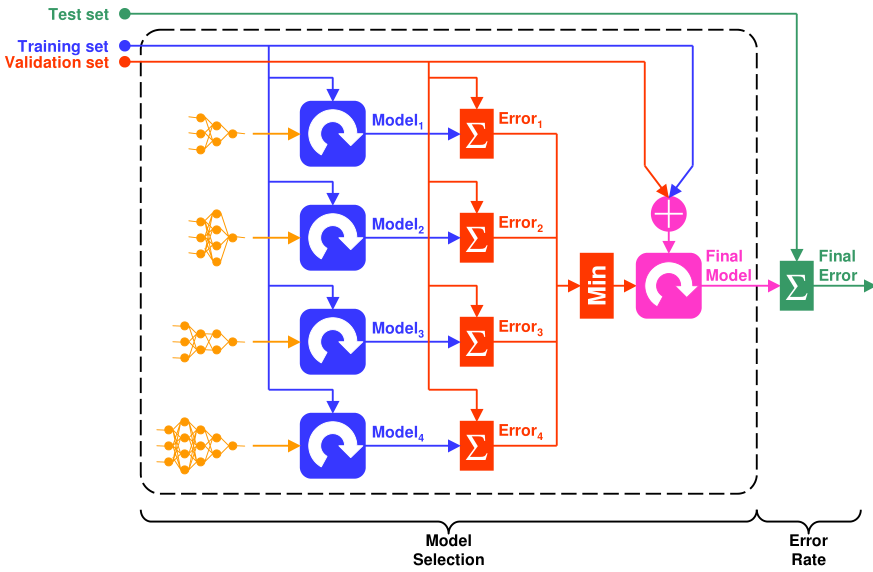
\includegraphics[width=.7\textwidth]{../report/resources/images/full-validation}
\end{frame}

\end{document}